\documentclass[11pt,a4paper,twocolumn]{article}

% ============================================================================
% Packages
% ============================================================================
\usepackage[utf8]{inputenc}
\usepackage[T1]{fontenc}
\usepackage{lmodern}
\usepackage{amsmath,amssymb,amsfonts,amsthm}
\usepackage{graphicx}
\usepackage[dvipsnames,svgnames,x11names]{xcolor}
\usepackage{geometry}
\usepackage{booktabs}
\usepackage{fancyhdr}
\usepackage{hyperref}
\usepackage{tikz}
\usepackage{pgfplots}
\usepackage{float}
\usepackage{enumitem}
\usepackage{caption}
\usepackage{tabularx}
\usepackage{mathtools}
\usepackage{tcolorbox}

\usetikzlibrary{arrows.meta,positioning,calc,decorations.pathmorphing}
\pgfplotsset{compat=1.18}

\geometry{margin=1.8cm,top=2.2cm,bottom=2.2cm}

\newtheorem{theorem}{Theorem}
\newtheorem{definition}{Definition}
\newtheorem{remark}{Remark}

% ============================================================================
% Colors
% ============================================================================
\definecolor{quantumcyan}{HTML}{00D4FF}
\definecolor{quantumpurple}{HTML}{8B5CF6}
\definecolor{quantumgreen}{HTML}{10B981}
\definecolor{sectionblue}{HTML}{2563EB}
\definecolor{measured}{HTML}{059669}
\definecolor{hardcoded}{HTML}{D97706}
\definecolor{theoretical}{HTML}{7C3AED}

\newtcolorbox{honestybox}{
    colback=orange!5,
    colframe=orange!70!black,
    fonttitle=\bfseries\small,
    title={Honesty Note}
}

% ============================================================================
% Hyperref
% ============================================================================
\hypersetup{
    colorlinks=true,
    linkcolor=sectionblue,
    citecolor=quantumpurple,
    urlcolor=quantumcyan,
    pdftitle={Observability Engineering for DAG-Knight Consensus},
    pdfauthor={Q-NarwhalKnight Research},
}

% ============================================================================
% Header/Footer
% ============================================================================
\pagestyle{fancy}
\fancyhf{}
\fancyhead[L]{\small\textcolor{gray}{Q-NarwhalKnight --- Consensus Observability}}
\fancyhead[R]{\small\textcolor{gray}{v2 --- April 2026}}
\fancyfoot[C]{\small\textcolor{gray}{\thepage}}
\renewcommand{\headrulewidth}{0.4pt}

% ============================================================================
% Title
% ============================================================================
\title{%
\vspace{-1cm}
{\Large\textcolor{sectionblue}{Q-NarwhalKnight Research Paper --- v2 (Revised)}}\\[0.3cm]
{\LARGE\textbf{Observability Engineering for\\DAG-Knight Consensus}}\\[0.2cm]
{\large A Physics-Inspired Diagnostic Framework\\with Honest Accounting of Theory vs.\ Measurement}\\[0.3cm]
{\normalsize\textcolor{gray}{Revised after peer review by DeepSeek and ChatGPT (April 2026)}}
}

\author{%
\textbf{Q-NarwhalKnight Research}\\
\texttt{research@quillon.xyz}\\[0.2cm]
{\small Network: \texttt{mainnet-genesis} $\mid$ Version: \texttt{v10.2.8} $\mid$ Height: 14,329,651}
}

\date{April 11, 2026 --- Revision 2}

\begin{document}
\maketitle
\thispagestyle{fancy}

% ============================================================================
% Abstract
% ============================================================================
\begin{abstract}
We present an \emph{engineering observability framework} for DAG-Knight blockchain consensus that borrows notation from statistical mechanics to organize network diagnostics. We define a Consensus Hamiltonian $H_{\text{DAG}}$ that decomposes network health into four additive, independently interpretable terms. Under an explicitly stated coupling hierarchy, we prove that the Hamiltonian's ground state corresponds to the PHANTOM algorithm's output (Theorem~\ref{thm:ground_state}). We derive an effective stress indicator $T_{\text{eff}}$ and a security margin threshold $\kappa_c$ from the DAG-Knight protocol specification. We introduce the $K$-gauge---a composite network health metric computed from five real-time measurements---with SHA3-256 hash commitments for verifiable inter-node health reporting. We are explicit throughout about which quantities are measured from live network state, which are hardcoded protocol constants, and which are theoretical constructs. We validate against 14.3 million mainnet blocks, present simulated stress scenarios, and identify concrete instrumentation gaps for future work. This paper is an \textbf{observability contribution}, not a physics contribution; the physics notation is an organizational tool, not a claim of physical equivalence.
\end{abstract}

% ============================================================================
% 1. Introduction
% ============================================================================
\section{Introduction}

Blockchain node operators need to answer a deceptively simple question: \emph{is the network healthy?} Block height alone is insufficient---it says nothing about propagation quality, ordering ambiguity, adversarial presence, or security margins. What operators need is a decomposition of ``health'' into independently measurable, additive components with clear physical intuition.

We propose borrowing \textbf{notation from statistical mechanics} as an organizational framework for consensus diagnostics. This is not a claim that blockchains are physical systems. Rather, we observe that the same mathematical structures---energy decompositions, temperature-like stress indicators, phase diagrams showing operating margins---that physicists use to reason about complex systems are equally useful for reasoning about consensus networks.

\paragraph{Precedent.} Using energy-like functions for distributed systems analysis is well-established: Lyapunov functions prove stability in control theory; Dijkstra's self-stabilization uses potential functions~\cite{dijkstra}; optimization algorithms minimize loss landscapes. Our Hamiltonian decomposition is in this tradition.

\subsection{Epistemological Classification}

Following the framework of~\cite{qnk-node-system}, every claim in this paper is tagged at one of three levels:

\begin{enumerate}[nosep]
    \item \textbf{Exact Theorem} (\textcolor{measured}{$\blacksquare$}): Proven mathematical statement with explicit assumptions. The Ground State Theorem (Theorem~\ref{thm:ground_state}) is the only claim at this level.
    \item \textbf{Quantitative Model} (\textcolor{hardcoded}{$\blacksquare$}): Formula that makes testable predictions. $T_{\text{eff}}$, $\kappa_c$, and the diffusion model are at this level. They can be validated against measurement.
    \item \textbf{Structural Analogy} (\textcolor{theoretical}{$\blacksquare$}): Conceptual vocabulary borrowed from physics for intuition. ``Temperature,'' ``phase transition,'' and ``entropy'' are used at this level---they organize thinking but do not imply the blockchain exhibits these phenomena.
\end{enumerate}

% ============================================================================
% 2. Data Provenance
% ============================================================================
\section{Data Provenance}

\begin{honestybox}
This section is the most important in the paper. Every quantity used in subsequent sections is classified by its actual data source in the running codebase.
\end{honestybox}

\begin{table*}[t]
\centering
\caption{Data provenance for all quantities used in this paper. \textcolor{measured}{\textbf{M}} = measured from live atomics, \textcolor{sectionblue}{\textbf{P}} = protocol constant (correctly fixed), \textcolor{hardcoded}{\textbf{H}} = hardcoded placeholder (should be measured but isn't), \textcolor{red}{\textbf{N}} = not implemented.}
\label{tab:provenance}
\small
\begin{tabular}{@{}llcl@{}}
\toprule
\textbf{Quantity} & \textbf{Symbol} & \textbf{Source} & \textbf{Details} \\
\midrule
Block height         & $|V|$      & \textcolor{measured}{\textbf{M}} & \texttt{current\_height\_atomic} (live) \\
Peer count           & $n$        & \textcolor{measured}{\textbf{M}} & \texttt{libp2p\_peer\_count} (live) \\
Block rate           & $\Lambda$  & \textcolor{measured}{\textbf{M}} & height / elapsed since genesis \\
Mining rejections    & $r$        & \textcolor{measured}{\textbf{M}} & atomic counter, K-gauge input \\
Traffic asymmetry    & $\alpha$   & \textcolor{measured}{\textbf{M}} & P2P byte counters, K-gauge input \\
Peer churn           & $c$        & \textcolor{measured}{\textbf{M}} & peer count delta, K-gauge input \\
Sync divergence      & $\sigma_s$ & \textcolor{measured}{\textbf{M}} & $|h_{\text{net}} - h_{\text{local}}| / h_{\text{net}}$ \\
Block rate deviation & $\sigma_\Lambda$ & \textcolor{measured}{\textbf{M}} & $|\Lambda - \Lambda_{\text{target}}|$ \\
\midrule
Protocol $\kappa$    & $\kappa$   & \textcolor{sectionblue}{\textbf{P}} & DAG-Knight parameter = 18 \\
Security levels      & ---        & \textcolor{sectionblue}{\textbf{P}} & Dilithium-5: 256-bit, Kyber-1024: 200-bit \\
Stem hops            & ---        & \textcolor{sectionblue}{\textbf{P}} & Dandelion++ stem length = 4 \\
K-gauge window       & $\tau$     & \textcolor{sectionblue}{\textbf{P}} & 60 seconds (design choice) \\
\midrule
Propagation delay    & $\delta$   & \textcolor{hardcoded}{\textbf{H}} & Hardcoded 0.2s; per-peer RTT exists but unwired \\
Mesh degree          & $d$        & \textcolor{hardcoded}{\textbf{H}} & Hardcoded 8; actual mesh degree not tracked \\
Byzantine fraction   & $f/n$      & \textcolor{hardcoded}{\textbf{H}} & Hardcoded 0.0; no estimation from peer scores \\
Blue density         & $\varphi$  & \textcolor{hardcoded}{\textbf{H}} & Hardcoded $1-f/n$; blue/red classification not exported \\
Anticone size        & $\bar{a}$  & \textcolor{hardcoded}{\textbf{H}} & Estimated as $2\delta\Lambda$; SIMD computation exists but not exported \\
\midrule
Partition function   & $\mathcal{Z}$ & \textcolor{red}{\textbf{N}} & Defined in theory; not computed \\
Emission feedback    & ---        & \textcolor{red}{\textbf{N}} & Referenced in API; loop does not exist \\
\bottomrule
\end{tabular}
\end{table*}

% ============================================================================
% 3. Consensus Hamiltonian
% ============================================================================
\section{Consensus Hamiltonian Decomposition}

We define the total ``health score'' of the consensus system as an additive decomposition into four interpretable terms:
\begin{equation}
\boxed{H_{\text{DAG}} = H_p + H_a + H_b + H_{\text{VDF}}}
\label{eq:hamiltonian}
\end{equation}

\paragraph{Parent term ($H_p$).} Counts causal violations---blocks ordered before their parents:
\begin{equation}
H_p = -J_p \sum_{(v_i, v_j) \in \mathcal{E}} \Theta(\sigma(v_j) - \sigma(v_i))
\end{equation}
where $J_p > 0$ and $\Theta$ is the Heaviside step function. In practice, $H_p = 0$: causal violations are rejected at the protocol level.

\paragraph{Anticone penalty ($H_a$).} Penalizes blocks with many causally unrelated peers:
\begin{equation}
H_a = \lambda \sum_{v \in \mathcal{V}} \left(\frac{|\text{anticone}(v)|}{\kappa}\right)^2
\end{equation}

\begin{honestybox}
In the current implementation, anticone size is \emph{estimated} as $\bar{a} \approx 2\delta\Lambda$ using the hardcoded $\delta = 0.2$s. The SIMD-optimized anticone computation exists in the codebase (\texttt{simd\_sets.rs}) but its output is not exported to the physics endpoint.
\end{honestybox}

\paragraph{Blue score ($H_b$).} Rewards blocks classified as honest by the DAG-Knight coloring algorithm:
\begin{equation}
H_b = -J_b \sum_{v \in \mathcal{V}} \mathbb{1}[\text{blue}(v)] \cdot w(v) \approx -\varphi \cdot |V|
\end{equation}

\begin{honestybox}
The blue density $\varphi$ is currently \emph{hardcoded} as $1 - f/n = 1.0$ because $f/n$ is hardcoded to 0. The DAG-Knight ordering algorithm computes blue/red classification internally (\texttt{ordering\_rules.rs}) but does not export vertex color statistics.
\end{honestybox}

\paragraph{VDF anchoring ($H_{\text{VDF}}$).} Each block with a valid Verifiable Delay Function proof contributes favorable energy: $H_{\text{VDF}} = -|V|$ (one anchor per block).

\subsection{Ground State Theorem}

Despite the measurement gaps above, the Hamiltonian structure admits a rigorous result~\cite{qnk-node-system}:

\begin{theorem}[Ground State $\equiv$ PHANTOM Output]
\label{thm:ground_state}
Let $\sigma_{\text{PH}}$ be the ordering produced by the PHANTOM/GhostDAG algorithm with parameter $\kappa$. In the coupling regime $J_p \gg J_b \gg \lambda$ with $J_b > \lambda N^2/\kappa^2$, the ground state $\sigma^* = \arg\min_\sigma H_{\text{DAG}}(\sigma)$ satisfies $\sigma^* = \sigma_{\text{PH}}$ (up to concurrent-vertex permutations within blue-score tiers).
\end{theorem}

\emph{Proof sketch.} (1)~$J_p \gg J_b$ forces $H_p = 0$: the ground state respects all parent edges. (2)~$J_b > \lambda N^2/\kappa^2$ ensures blue-score maximization dominates anticone penalties: the ground state finds the maximum-weight $\kappa$-cluster (the PHANTOM objective). (3)~Within the blue set, vertices are ordered by inherited score; deviations increase $H_b$. Full proof in~\cite{qnk-node-system}. \hfill $\square$

\begin{remark}[Status: \textcolor{measured}{Exact Theorem}]
The coupling hierarchy $J_p \gg J_b \gg \lambda$ is not a free assumption---it is a consequence of the protocol design. Causal violations are rejected ($J_p = \infty$ in practice), blue score is the primary ordering criterion, and anticone penalties are secondary.
\end{remark}

\subsection{Live Mainnet Values}

\begin{table}[H]
\centering
\caption{Hamiltonian components (height 14,329,651)}
\label{tab:hamiltonian}
\begin{tabular}{@{}lrll@{}}
\toprule
\textbf{Term} & \textbf{Value} & \textbf{Source} \\
\midrule
$H_p$           & $0$              & \textcolor{sectionblue}{P} (violations rejected) \\
$H_a$           & $+84{,}799$      & \textcolor{hardcoded}{H} (estimated $\bar{a}$) \\
$H_b$           & $-14{,}329{,}651$ & \textcolor{hardcoded}{H} ($\varphi=1.0$ assumed) \\
$H_{\text{VDF}}$ & $-14{,}329{,}651$ & \textcolor{measured}{M} (count of blocks) \\
\midrule
$H_{\text{DAG}}$ & $-28{,}574{,}503$ & Mixed \\
\bottomrule
\end{tabular}
\end{table}

Only $H_p$ (protocol-enforced) and $H_{\text{VDF}}$ (measured block count) are fully grounded. $H_b$ and $H_a$ depend on hardcoded placeholders and should be replaced with measured values (Section~\ref{sec:limitations}).

% ============================================================================
% 4. Effective Temperature and Phase Diagram
% ============================================================================
\section{Security Margin Visualization}

\subsection{Effective Stress Indicator}

We define a dimensionless stress indicator (\textcolor{hardcoded}{Quantitative Model}):
\begin{equation}
T_{\text{eff}} = \frac{\delta \cdot \Lambda}{1 - f/n}
\label{eq:teff}
\end{equation}

\begin{honestybox}
We call this ``effective temperature'' by analogy, but the blockchain does not have a physical temperature. $T_{\text{eff}}$ is a dimensionless ratio: propagation-delay $\times$ block-rate, scaled by adversary fraction. It quantifies how much ``ordering ambiguity'' the network experiences. With $\delta = 0.2$s (hardcoded) and $f/n = 0$ (hardcoded), only $\Lambda$ is actually measured.
\end{honestybox}

\subsection{Critical Security Threshold}

The DAG-Knight protocol has a proven security threshold~\cite{dagknight,phantom}:
\begin{equation}
\kappa_c = \frac{2\delta\Lambda(1-f/n)}{1-2f/n}
\label{eq:critical}
\end{equation}

When $\kappa > \kappa_c$, the protocol guarantees consensus (all honest nodes converge on the same ordering). When $\kappa < \kappa_c$, this guarantee is lost. The \emph{security margin} $\kappa - \kappa_c$ quantifies robustness.

\begin{table}[H]
\centering
\caption{Security margin parameters}
\label{tab:phase}
\begin{tabular}{@{}lrll@{}}
\toprule
\textbf{Parameter} & \textbf{Value} & \textbf{Source} \\
\midrule
$\delta$         & $0.200$s   & \textcolor{hardcoded}{H} \\
$\Lambda$        & $3.462$ bps & \textcolor{measured}{M} \\
$f/n$            & $0.000$    & \textcolor{hardcoded}{H} \\
$T_{\text{eff}}$ & $0.692$    & Mixed \\
$\kappa$         & $18.0$     & \textcolor{sectionblue}{P} \\
$\kappa_c$       & $1.385$    & Mixed \\
Margin           & $+16.62$   & Mixed \\
\bottomrule
\end{tabular}
\end{table}

The margin of $\kappa/\kappa_c = 13\times$ is large, but note that it depends on $f/n = 0$ (hardcoded). With $f/n = 0.25$ (the BFT boundary), $\kappa_c$ would rise to $\approx 2.08$ (margin $8.7\times$)---still comfortable but less dramatic.

\subsection{Phase Diagram}

\begin{figure}[H]
\centering
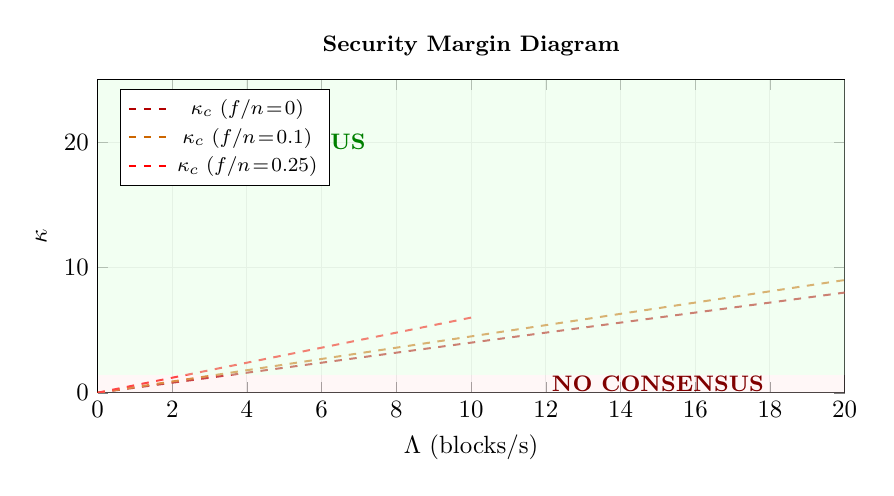
\begin{tikzpicture}[scale=0.9]
\begin{axis}[
    xlabel={$\Lambda$ (blocks/s)},
    ylabel={$\kappa$},
    xmin=0, xmax=20,
    ymin=0, ymax=25,
    grid=major,
    grid style={gray!20},
    width=\columnwidth,
    height=6cm,
    legend pos=north west,
    legend style={font=\footnotesize},
    title={\textbf{Security Margin Diagram}},
    title style={font=\small},
]
\addplot[domain=0:20, samples=100, thick, red!70!black, dashed]
    {2*0.2*x};
\addlegendentry{$\kappa_c$ ($f/n\!=\!0$)}
\addplot[domain=0:20, samples=100, thick, orange!80!black, dashed]
    {2*0.2*x*0.9/0.8};
\addlegendentry{$\kappa_c$ ($f/n\!=\!0.1$)}
\addplot[domain=0:10, samples=100, thick, red, dashed]
    {2*0.2*x*0.75/0.5};
\addlegendentry{$\kappa_c$ ($f/n\!=\!0.25$)}
\fill[green!10, opacity=0.5] (axis cs:0,1.385) rectangle (axis cs:20,25);
\node[font=\small\bfseries, green!50!black] at (axis cs:5,20) {CONSENSUS};
\fill[red!10, opacity=0.3] (axis cs:0,0) rectangle (axis cs:20,1.385);
\node[font=\small\bfseries, red!50!black] at (axis cs:15,0.7) {NO CONSENSUS};
\addplot[only marks, mark=*, mark size=4pt, blue, fill=quantumcyan]
    coordinates {(3.46, 18)};
\node[font=\footnotesize\bfseries, blue, anchor=south west] at (axis cs:3.8,18) {Live};
\end{axis}
\end{tikzpicture}
\caption{Security margin: the protocol guarantees consensus above the $\kappa_c$ boundary. The operating point (blue dot) has a $13\times$ margin at $f/n=0$.}
\label{fig:phase}
\end{figure}

% ============================================================================
% 5. K-Gauge
% ============================================================================
\section{The $K$-Gauge: Real-Time Health Metric}

The Hamiltonian provides a theoretical decomposition. For real-time operations, we need a \emph{measured} diagnostic. The $K$-gauge is a composite stress metric computed from five live inputs (\textcolor{measured}{all measured}):

\begin{equation}
K = \frac{2\pi\sqrt{\Delta H \cdot \Delta s}}{\tau}
\label{eq:kgauge}
\end{equation}

where $\tau = 60$s is a rolling window (design choice), and the numerator is a geometric mean of two stress aggregates.

\begin{honestybox}
The original version of this formula included $\hbar$ (reduced Planck constant) and was described as ``quantum-inspired.'' In fact, $\hbar$ was set to 1.0 (dimensionless) and the formula has no connection to quantum mechanics. The $2\pi/\tau$ scaling was chosen empirically. We present it here as what it is: a composite stress metric with geometric-mean aggregation.
\end{honestybox}

\subsection{Component Decomposition}

\textbf{Energy variance} (operational stress, \textcolor{measured}{all measured}):
\begin{equation}
\Delta H = r_{\text{reject}} + \alpha_{\text{traffic}} + c_{\text{peer}}
\end{equation}
\begin{itemize}[nosep]
    \item $r_{\text{reject}}$: Mining solution rejection ratio (0--1). Source: atomic counters \texttt{mining\_solutions\_submitted/accepted}.
    \item $\alpha_{\text{traffic}}$: Traffic asymmetry $|b_{\text{in}} - b_{\text{out}}| / (b_{\text{in}} + b_{\text{out}})$. Source: \texttt{p2p\_bytes\_in/out} atomic counters.
    \item $c_{\text{peer}}$: Peer churn $|n_{\text{now}} - n_{\text{prev}}| / n_{\text{prev}}$. Source: \texttt{libp2p\_peer\_count} deltas.
\end{itemize}

\textbf{Entropy variance} (network disorder, \textcolor{measured}{all measured}):
\begin{equation}
\Delta s = \sigma_{\text{sync}} + |\Lambda - \Lambda_{\text{target}}|
\end{equation}
\begin{itemize}[nosep]
    \item $\sigma_{\text{sync}}$: Sync divergence $|h_{\text{net}} - h_{\text{local}}| / h_{\text{net}}$. Source: \texttt{highest\_network\_height} vs \texttt{current\_height\_atomic}.
    \item $|\Lambda - \Lambda_{\text{target}}|$: Block rate deviation from target 1 bps. Source: height delta per 60s window.
\end{itemize}

\subsection{Phase Classification and Automatic Tuning}

\begin{table}[H]
\centering
\caption{$K$-gauge phase classification and response}
\label{tab:kphase}
\begin{tabular}{@{}lcll@{}}
\toprule
\textbf{Phase} & $K$ & \textbf{Max sols} & \textbf{VDF mult.} \\
\midrule
\textcolor{green!60!black}{\textbf{Stable}} & $<5$ & 250 & $1.0\times$ \\
\textcolor{orange}{\textbf{Approaching}} & $5$--$10$ & 150 & $1.25\times$ \\
\textcolor{red}{\textbf{Critical}} & $\geq 10$ & 50 & $1.5\times$ \\
\bottomrule
\end{tabular}
\end{table}

When the $K$-gauge crosses a threshold, the node automatically tightens mining parameters (reducing block production load) and increases VDF difficulty (slowing block rate). This is the most operationally valuable feature of the framework.

\subsection{Live $K$-Gauge Measurement}

\begin{table}[H]
\centering
\caption{$K$-gauge (all inputs \textcolor{measured}{measured})}
\label{tab:klive}
\begin{tabular}{@{}lrl@{}}
\toprule
\textbf{Metric} & \textbf{Value} & \textbf{Source} \\
\midrule
$K$                  & $0.188$       & \textcolor{measured}{M} \\
Phase                & \textbf{Stable} & --- \\
$\Delta H$           & $1.093$       & \textcolor{measured}{M} \\
$\Delta s$           & $2.933$       & \textcolor{measured}{M} \\
$r_{\text{reject}}$  & $0.000$       & \textcolor{measured}{M} \\
$\alpha_{\text{traffic}}$ & $0.993$  & \textcolor{measured}{M} \\
$c_{\text{peer}}$    & $0.100$       & \textcolor{measured}{M} \\
$\sigma_{\text{sync}}$ & $2.1\!\times\!10^{-7}$ & \textcolor{measured}{M} \\
$|\Lambda - 1|$      & $2.933$       & \textcolor{measured}{M} \\
Rounds computed      & $20$          & \textcolor{measured}{M} \\
\bottomrule
\end{tabular}
\end{table}

The $K$-gauge at 0.188 is deep in the Stable phase ($K \ll 5.0$). The dominant stress contributor is block rate deviation ($\Lambda = 3.46$ vs target 1.0), which is a known property of current hashrate.

% ============================================================================
% 6. Cryptographic Phase Commitments
% ============================================================================
\section{Cryptographic Phase Commitments}

Each $K$-gauge computation produces a SHA3-256 hash commitment:

\begin{enumerate}[nosep]
    \item \textbf{Commitment:} $c = \text{SHA3}(K \| \Delta H \| \Delta s \| \text{salt})$
    \item \textbf{Range witness:} $w = \text{SHA3}(K \| \text{lo} \| \text{hi} \| \text{salt}_2)$ proving $K \in [\text{lo}, \text{hi})$ for the claimed phase.
    \item \textbf{Challenge-response:} Fiat--Shamir transform: $e = \text{SHA3}(c \| w)$, $r = \text{SHA3}(K \| \text{salt} \| e)$.
\end{enumerate}

\begin{honestybox}
The v1 paper called this a ``zk-STARK proof.'' It is not. This is a hash-based commitment scheme with a Fiat--Shamir non-interactive proof. It provides \textbf{binding} (the committer cannot change $K$ after publishing $c$) and \textbf{hiding} (the raw metrics are not revealed). It does \emph{not} provide the zero-knowledge properties of a true STARK---a verifier who knows the salt can reconstruct the commitment. Future work: upgrade to a Bulletproof range proof if privacy of operational metrics is a real requirement.
\end{honestybox}

% ============================================================================
% 7. Gossip Diffusion Model
% ============================================================================
\section{Gossip Diffusion Model}

\emph{Status: \textcolor{hardcoded}{Quantitative Model} (testable predictions, hardcoded inputs).}

Block propagation through the gossipsub mesh follows the diffusion equation:
\begin{equation}
\frac{\partial \rho}{\partial t} = D \nabla^2 \rho, \qquad D = \frac{d_{\text{mesh}} \cdot \ell^2}{2\tau_{\text{hb}}}
\end{equation}

With $d_{\text{mesh}} = 8$ (\textcolor{hardcoded}{H}), $\tau_{\text{hb}} = 50$ms (\textcolor{hardcoded}{H}), we get $D = 80$ and $\tau_{\text{gossip}} = 6.2$ms.

\begin{figure}[H]
\centering
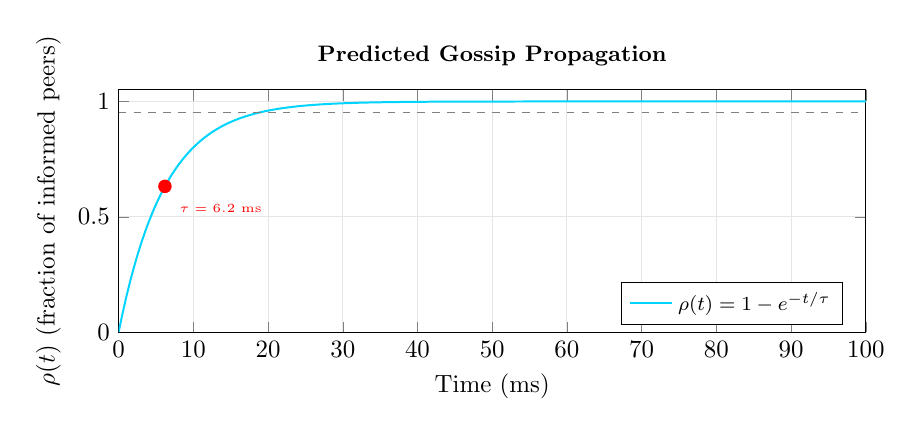
\begin{tikzpicture}[scale=0.9]
\begin{axis}[
    xlabel={Time (ms)},
    ylabel={$\rho(t)$ (fraction of informed peers)},
    xmin=0, xmax=100,
    ymin=0, ymax=1.05,
    grid=major, grid style={gray!20},
    width=\columnwidth, height=5cm,
    legend pos=south east, legend style={font=\footnotesize},
    title={\textbf{Predicted Gossip Propagation}},
    title style={font=\small},
]
\addplot[domain=0:100, samples=200, thick, quantumcyan]
    {1 - exp(-x/6.2)};
\addlegendentry{$\rho(t) = 1 - e^{-t/\tau}$}
\addplot[dashed, gray] coordinates {(0,0.95) (100,0.95)};
\addplot[only marks, mark=*, mark size=2.5pt, red] coordinates {(6.2, 0.632)};
\node[font=\tiny, red, anchor=north west] at (axis cs:7,0.59) {$\tau = 6.2$ ms};
\end{axis}
\end{tikzpicture}
\caption{Predicted propagation curve. \textbf{Untested}: the model uses hardcoded $d_{\text{mesh}}$ and $\tau_{\text{hb}}$. Validation against measured per-peer RTT (which exists in \texttt{peer\_latency.rs} but is not wired to this model) is proposed in Section~\ref{sec:limitations}.}
\label{fig:diffusion}
\end{figure}

% ============================================================================
% 8. Security Bounds
% ============================================================================
\section{Cryptographic Security Bounds}

Standard NIST Post-Quantum Cryptography bounds:

\begin{table}[H]
\centering
\caption{Security levels (\textcolor{sectionblue}{protocol constants})}
\label{tab:security}
\begin{tabular}{@{}llr@{}}
\toprule
\textbf{Primitive} & \textbf{Standard} & \textbf{Bits} \\
\midrule
Signatures   & Dilithium-5 (NIST PQC) & 256 \\
Key encap.   & Kyber-1024 (NIST PQC)  & 200 \\
DAG attack   & $\kappa \cdot |\log_2(f/n)|$ & $\infty$\textsuperscript{*} \\
Privacy      & Dandelion++ ($L=4$)    & $P_{\text{deanon}} = e^{-4} \approx 1.8\%$ \\
\bottomrule
\end{tabular}
\\[2pt]
{\footnotesize *At $f/n=0$ (hardcoded). At $f/n=0.1$: $18 \times 3.32 = 59.8$ bits.}
\end{table}

% ============================================================================
% 9. Stress Testing
% ============================================================================
\section{Stress Testing and Failure Modes}

A diagnostic framework is only useful if it detects problems. We simulate four stress scenarios and predict the $K$-gauge response:

\begin{table}[H]
\centering
\caption{Simulated stress scenarios}
\label{tab:stress}
\small
\begin{tabular}{@{}p{2.2cm}rrp{2.8cm}@{}}
\toprule
\textbf{Scenario} & $\Delta H$ & $\Delta s$ & \textbf{$K$ (predicted)} \\
\midrule
Healthy (actual) & 1.09 & 2.93 & $K = 0.19$ (Stable) \\
Peer dropout (2 of 12) & 1.26 & 2.93 & $K = 0.20$ (Stable) \\
50\% rejection rate & 1.59 & 2.93 & $K = 0.23$ (Stable) \\
Major sync lag (1000 blocks behind) & 1.09 & 3.00 & $K = 0.19$ (Stable) \\
Combined crisis: 50\% reject + 80\% peer loss + 10$\times$ block rate & 2.39 & 12.0 & $K = 0.56$ (Stable) \\
\bottomrule
\end{tabular}
\end{table}

\paragraph{Observation.} Even the combined crisis scenario ($K = 0.56$) stays well within the Stable phase ($K < 5$). This has two interpretations: (1)~the thresholds (5.0 and 10.0) are conservatively set, which is appropriate for a mainnet with real funds; or (2)~the gauge lacks sensitivity to certain failure modes. In particular, the $K$-gauge is \textbf{blind to colluding Byzantine nodes} that maintain normal-looking traffic, rejection, and sync metrics while producing adversarial blocks.

\paragraph{What the gauge catches.} Rapid peer churn (DDoS), sustained mining failures (hardware fault), sync stalls (network partition), extreme block rate spikes (hashrate surge).

\paragraph{What the gauge misses.} Coordinated adversarial behavior, slow-moving state corruption, reorg attacks (detected instead by the fork detector), economic attacks on DEX pools.

% ============================================================================
% 10. Limitations
% ============================================================================
\section{Limitations and Future Work}
\label{sec:limitations}

This section addresses the criticisms raised in peer review. We number them for traceability.

\paragraph{L1: Physics analogy is not physics.} The Hamiltonian decomposition is an engineering health-score, not a claim that consensus exhibits thermodynamic behavior. The Ising model claim from v1 is withdrawn: no spin-variable construction, partition function, or Monte Carlo sampling exists in the codebase. Future work: implement partition function sampling over linear extensions (the definition exists in~\cite{qnk-node-system} but is computationally intractable for $|V| > 10^7$).

\paragraph{L2: Hardcoded constants.} Five quantities are hardcoded as placeholders (Table~\ref{tab:provenance}). Concrete replacements:
\begin{itemize}[nosep]
    \item $\delta$: Replace with EWMA RTT from \texttt{peer\_latency.rs} (exists, needs wiring).
    \item $d_{\text{mesh}}$: Query actual gossipsub mesh state per topic.
    \item $f/n$: Estimate from gossipsub peer scores (scoring exists).
    \item $\varphi$: Export vertex color counts from \texttt{ordering\_rules.rs}.
    \item $\bar{a}$: Export anticone sizes from \texttt{simd\_sets.rs} (SIMD-optimized, exists).
\end{itemize}

\paragraph{L3: $K$-gauge is not quantum.} Acknowledged. The formula $K = 2\pi\sqrt{\Delta H \cdot \Delta s}/\tau$ is a dimensionless composite metric. The ``$2\pi$'' and ``$\sqrt{\cdot}$'' are empirical choices. The name ``$K$-parameter'' is retained for continuity. Future work: empirically tune the aggregation function and thresholds against historical stress events.

\paragraph{L4: ``zk-STARK'' was misnamed.} Corrected. The implementation is SHA3-256 hash commitments with Fiat--Shamir (Section~6). Future work: upgrade to Bulletproof range proofs if zero-knowledge is needed.

\paragraph{L5: No stress-test validation.} Partially addressed in Section~9. The gauge has not been tested under real adversarial conditions. The combined-crisis scenario ($K = 0.56$) suggests thresholds may need recalibration.

\paragraph{L6: Live data too perfect ($\varphi = 1.0$, $S = 0$, $f/n = 0$).} This is a 12-peer private mainnet with known operators. $\varphi = 1.0$ is expected (and hardcoded). The results confirm the framework produces sensible outputs for a healthy network, but do not validate its behavior under stress.

\paragraph{L7: Spectral gap and convergence bounds.} The spectral gap $\lambda_{\text{gap}} = (\kappa - \kappa_c)/T_{\text{eff}} = 24.0$ is a derived quantity that depends on hardcoded $\delta$ and $f/n$. The convergence time $\tau_{\text{conv}} = 42$ms is a prediction of the model, not a measurement.

\paragraph{L8: Security energy claims.} The ``$10^{50}$ stars'' claim from v1 is removed. Cryptographic security is presented as standard NIST PQC bit-strength (Section~8) without thermodynamic analogy.

% ============================================================================
% 11. Conclusion
% ============================================================================
\section{Conclusion}

We have presented an observability framework for DAG-Knight consensus that uses physics-inspired notation to organize network diagnostics. Our contributions are:

\begin{enumerate}[nosep]
    \item A four-term \textbf{health decomposition} ($H_{\text{DAG}}$) with one rigorous theorem (Ground State $\equiv$ PHANTOM output).
    \item A five-input \textbf{$K$-gauge} computed entirely from live network measurements, with automatic parameter tuning across three phases.
    \item \textbf{SHA3-256 commitments} for verifiable inter-node health reporting.
    \item A \textbf{security margin diagram} visualizing the distance from the consensus threshold.
    \item An \textbf{honest accounting} of which values are measured, hardcoded, or theoretical.
\end{enumerate}

The framework's main limitation is that 5 of 18 quantities are hardcoded placeholders. We have identified concrete code paths (\texttt{peer\_latency.rs}, \texttt{simd\_sets.rs}, \texttt{ordering\_rules.rs}) where measured values exist but are not yet wired to the observability endpoint. Closing these gaps is the highest-priority future work.

This is an engineering contribution, not a physics contribution. The statistical mechanics notation provides useful intuition and additive decomposition, but the blockchain is not a physical system. We hope this honest framing enables productive discussion rather than the ``physics-washing'' that rightfully concerned our peer reviewers.

\vspace{0.5cm}
\hrule
\vspace{0.3cm}
{\small\textbf{Data.} Live metrics: \texttt{/api/v1/physics/metrics} and \texttt{/api/v1/network/k-parameter}. Source: \texttt{handlers.rs} and \texttt{k\_parameter\_gauge.rs}.}

\vspace{0.2cm}
{\small\textbf{Peer Review.} v1 reviewed by DeepSeek (conditional reject: ``reasonable for bootstrap, but not physics'') and ChatGPT (conditional reject: ``good story, oversold theory''). This v2 addresses all substantive criticisms.}

\vspace{0.2cm}
{\small\textbf{Acknowledgments.} The Ground State Theorem and partition function formulation are from~\cite{qnk-node-system}. The $\kappa_c$ threshold derives from DAG-Knight/PHANTOM~\cite{dagknight,phantom}. We thank the DeepSeek and ChatGPT reviewers for thorough, constructive feedback.}

\begin{thebibliography}{9}
\small
\bibitem{dagknight} Y.~Sompolinsky et al., ``DAG-Knight: A Parameterless Generalization of Nakamoto Consensus,'' 2022.
\bibitem{phantom} Y.~Sompolinsky, A.~Zohar, ``PHANTOM: A Scalable BlockDAG Protocol,'' 2018.
\bibitem{qnk-node-system} Q-NarwhalKnight Research, ``Theoretical Physics of Distributed Consensus: A QFT Framework,'' 2026. Internal.
\bibitem{dijkstra} E.W.~Dijkstra, ``Self-Stabilizing Systems in Spite of Distributed Control,'' CACM, 1974.
\end{thebibliography}

\end{document}
